\documentclass[11pt]{article}
\usepackage{amsmath}
\usepackage{amssymb}
\usepackage{graphicx}
\usepackage{tabularx}
\usepackage{fancyhdr}
\usepackage{lastpage}

% Page layout
\usepackage[top=1in, bottom=1in, left=1in, right=1in]{geometry}

% Header and footer
\pagestyle{fancy}
\fancyhf{}
\rfoot{Page \thepage}
\renewcommand{\headrulewidth}{0pt}

% Modified Question command with left-aligned number
\newcommand{\questiona}[2]{
    \noindent\textbf{Q#2.} #1 \hfill \textbf{[1 Mark]}
}

\newcommand{\questionb}[2]{
    \noindent\textbf{Q#2.} #1 \hfill \textbf{[2 Marks]}
}

\begin{document}

% Title section with horizontal line
\begin{center}
    \Large\textbf{GATE 2017 - Textile Engineering and Fibre Science (TF)} \\
    \large\textbf{General Aptitude and Technical Questions} \\
    \rule{\textwidth}{0.5pt} % Horizontal line below heading
\end{center}

\vspace{0.5cm}

% General Aptitude Section
\section*{General Aptitude}

\questiona{He was one of my best \_\_\_\_\_ and I felt his loss \_\_\_\_\_.}{1}
\begin{enumerate}
    \item[(A)] friend, keenly  
    \item[(B)] friends, keen  
    \item[(C)] friend, keener  
    \item[(D)] friends, keenly  
\end{enumerate}
\vspace{0.5cm}

\questiona{As the two speakers became increasingly agitated, the debate became \_\_\_\_\_.}{2}
\begin{enumerate}
    \item[(A)] lukewarm  
    \item[(B)] poetic  
    \item[(C)] forgiving  
    \item[(D)] heated  
\end{enumerate}
\vspace{0.5cm}

\questiona{A right-angled cone (with base radius 5 cm and height 12 cm), as shown in the figure below, is rolled on the ground keeping the point P fixed until the point Q (at the base of the cone, as shown) touches the ground again.}{3}
\begin{center}
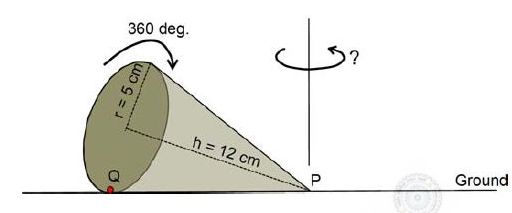
\includegraphics[width=0.5\textwidth]{figures/3.png}
\end{center}
By what angle (in radians) about P does the cone travel?
\begin{enumerate}
    \item[(A)] $\frac{5\pi}{12}$
    \item[(B)] $\frac{5\pi}{24}$
    \item[(C)] $\frac{24\pi}{5}$
    \item[(D)] $\frac{10\pi}{13}$
\end{enumerate}
\vspace{0.5cm}

\questiona{In a company with 100 employees, 45 earn Rs. 20,000 per month, 25 earn Rs. 30,000, 20 earn Rs. 40,000, 8 earn Rs. 60,000, and 2 earn Rs. 150,000. The median of the salaries is}{4}
\begin{enumerate}
    \item[(A)] Rs. 20,000
    \item[(B)] Rs. 30,000
    \item[(C)] Rs. 32,300
    \item[(D)] Rs. 40,000
\end{enumerate}
\vspace{0.5cm}

\questiona{P, Q, and R talk about S's car collection. P states that S has at least 3 cars. Q believes that S has less than 3 cars. R indicates that to his knowledge, S has at least one car. Only one of P, Q and R is right. The number of cars owned by S is}{5}
\begin{enumerate}
    \item[(A)] 0
    \item[(B)] 1
    \item[(C)] 3
    \item[(D)] Cannot be determined
\end{enumerate}
\vspace{0.5cm}

\questionb{"Here, throughout the early 1820s, Stuart continued to fight his losing battle to allow his sepoys to wear their caste-marks and their own choice of facial hair on parade, being again reprimanded by the commander-in-chief. His retort that 'A stronger instance than this of European prejudice with relation to this country has never come under my observations' had no effect on his superiors."
According to this paragraph, which of the statements below is most accurate?}{6}
\begin{enumerate}
    \item[(A)] Stuart's commander-in-chief was moved by this demonstration of his prejudice.
    \item[(B)] The Europeans were accommodating of the sepoys' desire to wear their caste-marks.
    \item[(C)] Stuart's 'losing battle' refers to his inability to succeed in enabling sepoys to wear caste-marks.
    \item[(D)] The commander-in-chief was exempt from the European prejudice that dictated how the sepoys were to dress.
\end{enumerate}
\vspace{0.5cm}

\questionb{What is the sum of the missing digits in the subtraction problem below?}{7}
\begin{center}
$\begin{array}{c}
5\ \_\ \_\ \_\ \_\ \_\ \_\ \\
-4\ \_\ 8\ \_\ \_\ 8\ \_\ 9 \\
\hline
1\ 1\ 1\ 1 \\
\end{array}$
\end{center}
\begin{enumerate}
    \item[(A)] 8  
    \item[(B)] 10  
    \item[(C)] 11  
    \item[(D)] Cannot be determined  
\end{enumerate}
\vspace{0.5cm}

\questionb{Let S$_1$ be the plane figure consisting of the points $(x, y)$ given by the inequalities $|x - 1| \leq 2$ and $|y + 2| \leq 3$. Let S$_2$ be the plane figure given by the inequalities $x - y \geq -2$, $y \geq 1$, and $x \leq 3$. Let S be the union of S$_1$ and S$_2$. The area of S is}{8}
\begin{enumerate}
    \item[(A)] 26  
    \item[(B)] 28  
    \item[(C)] 32  
    \item[(D)] 34  
\end{enumerate}
\vspace{0.5cm}

\questionb{Two very famous sportsmen Mark and Steve happened to be brothers, and played for country K. Mark teased James, an opponent from country E, "There is no way you are good enough to play for your country." James replied, "Maybe not, but at least I am the best player in my own family."
Which one of the following can be inferred from this conversation?}{9}
\begin{enumerate}
    \item[(A)] Mark was known to play better than James  
    \item[(B)] Steve was known to play better than Mark  
    \item[(C)] James and Steve were good friends  
    \item[(D)] James played better than Steve  
\end{enumerate}
\vspace{0.5cm}

% Technical Section
\section*{Technical Section}

\questiona{If the scalar projection of the vector \( \vec{a} = 3\hat{i} + \beta \hat{k} \) on the vector \( \vec{b} = 2\hat{i} - 2\hat{j} + \hat{k} \) is 5, then a value of \( \beta \) is equal to}{1}
\begin{enumerate}
    \item[(A)] 21  
    \item[(B)] 9  
    \item[(C)] -1  
    \item[(D)] -6  
\end{enumerate}
\vspace{0.5cm}

\questiona{The Laplace transform of \( e^{-t} \cos (2t) \) is}{2}
\begin{enumerate}
    \item[(A)] \( \frac{s-1}{s^2 - 2s + 5} \)  
    \item[(B)] \( \frac{1}{s^2 + 2s + 5} \)  
    \item[(C)] \( \frac{s+1}{s^2 + 2s + 2} \)  
    \item[(D)] \( \frac{s+1}{s^2 + 2s + 5} \)  
\end{enumerate}
\vspace{0.5cm}

\questiona{If \( z(x, y) = x^2 - y^2, x(t) = t - t^{-2} \) and \( y(t) = t^2 + t^{-3} \) then \( \frac{dz}{dt} \) at \( t = 1 \) is equal to \_\_\_\_\_.}{3}
\vspace{0.5cm}

\questiona{The characteristic observation in burning test of cotton fibre is}{4}
\begin{enumerate}
    \item[(A)] Burns readily with whitish ash as residue  
    \item[(B)] Burns with dripping  
    \item[(C)] Burns with burning hair smell  
    \item[(D)] Melts and forms a hard bead  
\end{enumerate}
\vspace{0.5cm}

\questiona{The given structure is a repeat unit of}{5}
\begin{center}
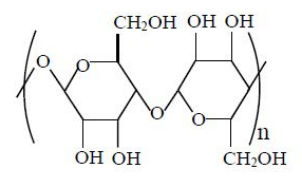
\includegraphics[width=0.5\textwidth]{figures/5.png}
\end{center}
\begin{enumerate}
    \item[(A)] Cellulose acetate  
    \item[(B)] Cellulose  
    \item[(C)] Polyamide  
    \item[(D)] Polyester  
\end{enumerate}
\vspace{0.5cm}

\questiona{Which of the following is(are) bast fibre(s)\\
P. Cotton \\ 
Q. Flax  \\
R. Silk  \\
S. Jute  }{6}
\begin{enumerate}
    \item[(A)] P only  
    \item[(B)] Q and R only  
    \item[(C)] Q and S only  
    \item[(D)] S only  
\end{enumerate}
\vspace{0.5cm}

\questiona{During crystallization of polyester}{7}
\begin{enumerate}
    \item[(A)] Heat is evolved  
    \item[(B)] Heat is absorbed  
    \item[(C)] No exchange of heat takes place  
    \item[(D)] Small molecule such as water is eliminated  
\end{enumerate}
\vspace{0.5cm}

\questiona{Which of the following fibre(s) is(are) manufactured by melt spinning process\\
P. Viscose \\ 
Q. Cellulose acetate  \\
R. Nylon-6 \\ 
S. Aramid  }{8}
\begin{enumerate}
    \item[(A)] P only  
    \item[(B)] Q and R only  
    \item[(C)] R only  
    \item[(D)] R and S only  
\end{enumerate}
\vspace{0.5cm}

\questiona{Keeping card production same, the quality of carding will improve by setting}{9}
\begin{enumerate}
    \item[(A)] Higher doffer rpm and coarser sliver hank  
    \item[(B)] Higher doffer rpm and finer sliver hank  
    \item[(C)] Lower doffer rpm and coarser sliver hank  
    \item[(D)] Lower doffer rpm and finer sliver hank  
\end{enumerate}
\vspace{0.5cm}

\questiona{The tenacity of\\
P. Carded sliver  \\
Q. First drawn sliver  \\
R. Second drawn sliver  \\
S. Combed sliver  
follows the order  }{10}
\begin{enumerate}
    \item[(A)] \( P > Q > R > S \)  
    \item[(B)] \( S > R > Q > P \)  
    \item[(C)] \( R > S > P > Q \)  
    \item[(D)] \( Q > R > S > P \)
\end{enumerate}
\vspace{0.5cm}

\questiona{For a given yarn fineness, use of ring traveller of too small a mass gives}{11}
\begin{enumerate}
    \item[(A)] Small balloon size but more yarn content on the bobbin  
    \item[(B)] Small balloon size but less yarn content on the bobbin  
    \item[(C)] Big balloon size but more yarn content on the bobbin  
    \item[(D)] Big balloon size but less yarn content on the bobbin  
\end{enumerate}
\vspace{0.5cm}

\questiona{In cotton combing process, the counter-feed system gives}{12}
\begin{enumerate}
    \item[(A)] Low removal of noil and low elimination of impurities  
    \item[(B)] Low removal of noil and high elimination of impurities  
    \item[(C)] High removal of noil and low elimination of impurities  
    \item[(D)] High removal of noil and high elimination of impurities  
\end{enumerate}
\vspace{0.5cm}

\questiona{Probability of warp breakage during weaving increases, when}{13}
\begin{enumerate}
    \item[(A)] Warp extensibility is decreased  
    \item[(B)] Warp unevenness is decreased  
    \item[(C)] End density is decreased  
    \item[(D)] Warp hairiness is decreased  
\end{enumerate}
\vspace{0.5cm}

\questiona{In terms of weft insertion rate, which of the following is correct?}{14}
\begin{enumerate}
    \item[(A)] $Airjet > Waterjet > Multiphase > Projectile$  
    \item[(B)] $Multiphase > Airjet > Waterjet > Projectile$  
    \item[(C)] $Projectile > Waterjet > Airjet > Multiphase$  
    \item[(D)] $Waterjet > Projectile > Multiphase > Airjet$  
\end{enumerate}
\vspace{0.5cm}

\questiona{A tuck stitch in knitting makes the fabric}{15}
\begin{enumerate}
    \item[(A)] Narrower  
    \item[(B)] Thinner  
    \item[(C)] More rigid in course direction  
    \item[(D)] Wider and porous  
\end{enumerate}
\vspace{0.5cm}

\questiona{A perpendicular-laid nonwoven}{16}
\begin{enumerate}
    \item[(A)] Should not contain thermoplastic fibre  
    \item[(B)] Does not form a 3-D structure  
    \item[(C)] Cannot be used as a replacement of foam  
    \item[(D)] Exhibits high recovery from compression  
\end{enumerate}
\vspace{0.5cm}

\questiona{The cut squaring technique of sampling of fibres is \textbf{NOT} applicable to}{17}
\begin{enumerate}
    \item[(A)] Bale  
    \item[(B)] Silver  
    \item[(C)] Roving  
    \item[(D)] Yarn  
\end{enumerate}
\vspace{0.5cm}

\questiona{The ratio of wet-strength to dry-strength of viscose fibre is}{18}
\begin{enumerate}
    \item[(A)] Equal to one  
    \item[(B)] Always less than one  
    \item[(C)] Always greater than one  
    \item[(D)] Sometimes greater and sometimes less than one  
\end{enumerate}
\vspace{0.5cm}

\questiona{Theoretical limit for mass irregularity (CV\(_{lim}\)) of a cotton yarn does \textbf{NOT} depend on}{19}
\begin{enumerate}
    \item[(A)] Mean fibre length  
    \item[(B)] Mean fibre fineness  
    \item[(C)] Mean yarn count  
    \item[(D)] Coefficient of variation of fibre fineness  
\end{enumerate}
\vspace{0.5cm}

\questiona{Diamond bars appear in woven fabric due to}{20}
\begin{enumerate}
    \item[(A)] Faulty loom parts  
    \item[(B)] Excessive warp irregularity  
    \item[(C)] Periodic fault in warp yarn  
    \item[(D)] Periodic fault in weft yarn  
\end{enumerate}
\vspace{0.5cm}

\questiona{In a three-sigma control chart, the probability that a point falls outside the control limits, when a process is under control, is}{21}
\begin{enumerate}
    \item[(A)] 0  
    \item[(B)] 0.0027  
    \item[(C)] 0.01  
    \item[(D)] 0.05  
\end{enumerate}
\vspace{0.5cm}

\questiona{Shrinkage of cotton fabric during wetting is caused by}{22}
\begin{enumerate}
    \item[(A)] Extension of fibre  
    \item[(B)] Crimping of fibre  
    \item[(C)] Swelling of fibre  
    \item[(D)] Compression of fibre  
\end{enumerate}
\vspace{0.5cm}

\questiona{Vapour-phase flame retardant agents are based on compounds containing}{23}
\begin{enumerate}
    \item[(A)] Nitrogen  
    \item[(B)] Phosphorus  
    \item[(C)] Halogens  
    \item[(D)] Aluminium  
\end{enumerate}
\vspace{0.5cm}

\questiona{White specks observed in dyed cotton fabric are attributed to}{24}
\begin{enumerate}
    \item[(A)] Poor wash fastness of dyes  
    \item[(B)] Non-uniform agitation of dye bath  
    \item[(C)] Low temperature of dyeing  
    \item[(D)] Presence of immature cotton fibres  
\end{enumerate}
\vspace{0.5cm}

\questiona{Number of moles, accurate to one decimal place, required in 200 cm\(^3\) to make 0.5 mol l\(^{-1}\) sodium hydroxide solution is \_\_\_\_\_.}{25}
\vspace{0.5cm}

\questionb{The median, accurate to two decimal places, of a random variable \( X \) with the probability density function
\[f(x) = 
\begin{cases} 
3x^{-4} & x > 1 \\ 
0 & x \leq 1, 
\end{cases}\]  
is \_\_\_\_\_.}{26}
\vspace{0.5cm}

\questionb{Using Simpson's 1/3 rule, the value of the integral
\[\frac{1}{\pi} \int_0^{\pi} \left( 1 + \sqrt{\sin(x)} \right) dx,\]  
accurate to two decimal places, is \_\_\_\_\_.}{27}
\vspace{0.5cm}

\questionb{If a solution curve of the differential equation
\[x \frac{dy}{dx} = y + 2x^3\]  
passes through the point (1, 0), then this curve also passes through the point}{28}
\begin{enumerate}
    \item[(A)] \((-1, 0)\)  
    \item[(B)] \((0, -1)\)  
    \item[(C)] \((2, 10)\)  
    \item[(D)] \((-2, 6)\)  
\end{enumerate}
\vspace{0.5cm}

\questionb{The system of linear equations
\[\begin{cases} 
\alpha x - 2y = 4 \\ 
2x + 4y = \beta 
\end{cases}\]  
has}{29}
\begin{enumerate}
    \item[(A)] No solution for \(\alpha = 1\), \(\beta = -8\)  
    \item[(B)] Unique solution for \(\alpha = -1\), \(\beta = 8\)  
    \item[(C)] Infinitely many solutions for \(\alpha = -1\), \(\beta = -8\)  
    \item[(D)] Infinitely many solutions for \(\alpha = 1\), \(\beta = 8\)
\end{enumerate}
\vspace{0.5cm}

\questionb{The function \( f(x) = x^3 - 3x^2 - 9x + 10 \) is}{30}
\begin{enumerate}
    \item[(A)] Increasing in the interval (1, \(\infty\))  
    \item[(B)] Increasing in the interval (\(-\infty\), 1)  
    \item[(C)] Decreasing in the interval (\(-1\), 3)  
    \item[(D)] Decreasing in the interval (\(-3\), 1)  
\end{enumerate}
\vspace{0.5cm}

\questionb{Group I contains techniques of fibre manufacturing. Group II gives the physical phenomena associated with these techniques. Match the technique with the phenomenon}{31}

\begin{center}
\begin{tabular}{|l|l|}
\hline
\textbf{Group I} & \textbf{Group II} \\
\hline
P. Melt spinning & 1. Diffusion of only solvent \\
Q. Wet spinning & 2. Diffusion of both solvent and non-solvent \\
R. Dry spinning & 3. No solvent diffusion \\
\hline
\end{tabular}
\end{center}

\begin{enumerate}
    \item[(A)] P-1, Q-2, R-3  
    \item[(B)] P-3, Q-1, R-2  
    \item[(C)] P-3, Q-2, R-1  
    \item[(D)] P-1, Q-3, R-2  
\end{enumerate}
\vspace{0.5cm}

\questionb{The average molecular mass, in g/mol, of nylon-6 polymer, having average degree of polymerization of 100, is \_\_\_\_\_.}{32}
\vspace{0.5cm}

\questionb{Group I consists of names of fibres. Group II gives characteristic structural features of these fibres. Match the fibre from Group I to its respective feature from Group II.}{33}

\begin{center}
\begin{tabular}{|l|l|}
\hline
\textbf{Group I} & \textbf{Group II} \\
\hline
P. Cotton & 1. Para- and ortho-cortex \\
Q. Jute & 2. Primary and secondary wall \\
R. Wool & 3. Fibroin \(\beta\)-sheets \\
S. Silk & 4. Multicellular \\
\hline
\end{tabular}
\end{center}

\begin{enumerate}
    \item[(A)] P-4, Q-1, R-2, S-3  
    \item[(B)] P-2, Q-4, R-1, S-3  
    \item[(C)] P-2, Q-3, R-4, S-1  
    \item[(D)] P-2, Q-4, R-3, S-1  
\end{enumerate}
\vspace{0.5cm}

\questionb{Wool gives warmth because it has\\
P. A helical structure which can entrap air \\ 
Q. High heat of sorption \\ 
R. Low crystallinity \\ 
S. High extensibility }{34} 
\begin{enumerate}
    \item[(A)] P and Q only  
    \item[(B)] Q and R only  
    \item[(C)] P and S only  
    \item[(D)] P and R only  
\end{enumerate}
\vspace{0.5cm}

\questionb{To obtain high molecular weight nylon-66, if 11.6 g of hexamethylene diamine (molecular weight 116 g/mol) is used, then the required amount of adipic acid (molecular weight 146 g/mol), in gram, accurate to one decimal place, is \_\_\_\_\_.}{35}
\vspace{0.5cm}

\questionb{If the distance between two adjacent fibres of circular cross-section in a hexagonally packed yarn is equal to the radius of the fibre, then the packing density of yarn, accurate to three decimal places, is \_\_\_\_\_.}{36}
\vspace{0.5cm}

\questionb{A 30 tex open-end rotor yarn having 650 twist per meter is produced using 33 mm rotor diameter and 1,20,000 rotor rpm. The rotational speed of the peel-off point is \_\_\_\_\_ \(\times 10^3\) rpm.}{37}
\vspace{0.5cm}

\questionb{A bobbin lead roving frame is running at 25 m/min delivery speed and 1250 rpm spindle speed. The rotational speed of the bobbin, at the instant of 0.10 m bobbin diameter, accurate to two decimal places, is \_\_\_\_\_ rpm.}{38}
\vspace{0.5cm}

\questionb{A T-shirt is produced from cotton fibre of 1520 kg/m\(^3\) density, 1.4 dtex fineness and 30 mm length. The total number of fibres in the T-shirt of 0.15 kg is \_\_\_\_\_ \(\times 10^6\).}{39}
\vspace{0.5cm}

\questionb{Pilling resistance of}{40}
\begin{enumerate}
    \item[(A)] Ring yarn is higher than open-end rotor yarn but lesser than air vortex yarn  
    \item[(B)] Air vortex yarn is higher than ring yarn but lesser than open-end rotor yarn  
    \item[(C)] Open-end rotor yarn is higher than ring yarn but lesser than air vortex yarn  
    \item[(D)] Ring yarn is higher than air vortex yarn but lesser than open-end rotor yarn  
\end{enumerate}
\vspace{0.5cm}

\questionb{A needle loom, having a needle board with 2000 needles/m, is operating at a stroke frequency of 2000 strokes/min and producing a needle-punched nonwoven fabric at 5 m/min. The punch density, in number of punches per cm\(^2\), is \_\_\_\_\_.}{41}
\vspace{0.5cm}

\questionb{Compared to conventional sizing, the wet sizing process reduces}{42}
\begin{enumerate}
    \item[(A)] Size consumption substantially  
    \item[(B)] Consumption of drying energy  
    \item[(C)] Weavability of warp yarn  
    \item[(D)] Tensile strength of yarn  
\end{enumerate}
\vspace{0.5cm}

\questionb{In a fabric, warp count is 25 tex, weft count is 32 tex, ends per cm is 25, picks per cm is 15, warp crimp is 6\% and weft crimp is 8\%. The areal density of the fabric, in g/m\(^2\), accurate to two decimal places, is \_\_\_\_\_.}{43}
\vspace{0.5cm}

\questionb{Let a cheese of 160 mm traverse length be wound on a rotary traverse machine having a drum of 75 mm diameter and 2.5 crossings. If the drum rotates at 3250 rpm, then the coil angle, in degrees, accurate to one decimal place, is \_\_\_\_\_.}{44}
\vspace{0.5cm}

\questionb{Group I consists of weave designs. Group II lists end-use / property. Match the weave design from Group I with the corresponding end-use / property from Group II}{45}

\begin{center}
\begin{tabular}{|l|l|}
\hline
\textbf{Group I} & \textbf{Group II} \\
\hline
P. Leno & 1. Furnishing \\
Q. Honeycomb & 2. Broken and irregular surface \\
R. Jacquard & 3. Mosquito net \\
S. Crepe & 4. Towel \\
\hline
\end{tabular}
\end{center}

\begin{enumerate}
    \item[(A)] P-3, Q-4, R-1, S-2  
    \item[(B)] P-4, Q-1, R-3, S-2  
    \item[(C)] P-1, Q-2, R-4, S-3  
    \item[(D)] P-3, Q-4, R-2, S-1  
\end{enumerate}
\vspace{0.5cm}

\questionb{At 65\% relative humidity and 20°C temperature, the moisture regain of the fibres\\
(P) Wool  \\
(Q) Nylon 6  \\
(R) Cotton  \\
(S) Polyester \\ 
follows the order  }{46}
\begin{enumerate}
    \item[(A)] \( P > Q > R > S \)  
    \item[(B)] \( P > R > Q > S \)  
    \item[(C)] \( R > P > Q > S \)  
    \item[(D)] \( R > P > S > Q \)  
\end{enumerate}
\vspace{0.5cm}

\questionb{While measuring tensile properties using Stelometer at 3.2 mm gauge length, a cotton fibre bundle of 15 mm length and 4.5 mg weight registers a breaking load of 6 kg. The bundle tenacity (g/tex) is \_\_\_\_\_.}{47}
\vspace{0.5cm}

\questionb{The tenacity of a two-fold yarn is 1.1 times the tenacity of its component single yarn. The breaking load of the two-fold yarn is X times the breaking load of its single component yarn. Neglecting length contraction due to twist, the value of X, accurate to one decimal place, is \_\_\_\_\_.}{48}
\vspace{0.5cm}

\questionb{The compressive pressure applied onto a fabric is inversely proportional to the cube of thickness of the fabric. If the thickness is halved during compression, then the pressure increases by \_\_\_\_\_ times.}{49}
\vspace{0.5cm}

\questionb{The coefficient of correlation between packing density and porosity of a set of yarns is \_\_\_\_\_.}{50}
\vspace{0.5cm}

\questionb{Determine the correctness or otherwise of the following Assertion [a] and the Reason [r] \\

Assertion: Jet dyeing machines yield level dyeing in short dyeing time \\ 
Reason: Jet dyeing machines use pressure jets to force dye into the fibre }{51} 

\begin{enumerate}
    \item[(A)] Both [a] and [r] are true, and [r] is the correct reason for [a]  
    \item[(B)] Both [a] and [r] are true, but [r] is not the correct reason for [a]  
    \item[(C)] Both [a] and [r] are false  
    \item[(D)] [a] is true but [r] is false  
\end{enumerate}
\vspace{0.5cm}

\questionb{Group I lists chemical processes. Group II lists chemicals used in these processes. Match the process with the corresponding chemical}{52}

\begin{center}
\begin{tabular}{|l|l|}
\hline
\textbf{Group I} & \textbf{Group II} \\
\hline
P. Carbonising & 1. Na\(_2\)CO\(_3\) \\
Q. Scouring & 2. H\(_2\)SO\(_4\) \\
R. Bleaching & 3. NaOH \\
S. Mercerising & 4. H\(_2\)O\(_2\) \\
\hline
\end{tabular}
\end{center}

\begin{enumerate}
    \item[(A)] P-2, Q-3, R-4, S-1  
    \item[(B)] P-2, Q-1, R-4, S-3  
    \item[(C)] P-3, Q-1, R-2, S-3  
    \item[(D)] P-2, Q-1, R-3, S-4  
\end{enumerate}
\vspace{0.5cm}

\questionb{Determine the correctness or otherwise of the following statements\\

p: The contact angle \(\theta\) is indicative of the wettability of a textile surface by a liquid  \\
q: Values of \(\theta > 90^\circ\) indicate poor wetting surfaces  }{53}

\begin{enumerate}
    \item[(A)] Both [p] and [q] are true  
    \item[(B)] Both [p] and [q] are false  
    \item[(C)] [p] is true but [q] is false  
    \item[(D)] [p] is false but [q] is true  
\end{enumerate}
\vspace{0.5cm}

\questionb{The add-on of a chemical finish required on a fabric is 3\% on-weight-of-fabric (owf). If the wet pick up is 80\%, then the concentration of finish required in the padding bath, in \% (wt/wt), accurate to two decimal places, is \_\_\_\_\_.}{54}
\vspace{0.5cm}

\questionb{Determine the correctness or otherwise of the following Assertion [a] and the Reason [r]\\

Assertion: Burnt out effect on polyester/cotton blend fabric can be obtained by printing  \\
Reason: Printing paste contains a reagent that releases an acid during steaming  }{55}

\begin{enumerate}
    \item[(A)] Both [a] and [r] are true and [r] is the correct reason for [a]  
    \item[(B)] Both [a] and [r] are true but [r] is not the correct reason for [a]  
    \item[(C)] Both [a] and [r] are false  
    \item[(D)] [a] is true but [r] is false  
\end{enumerate}
\vspace{0.5cm}

\begin{center}
\textbf{END OF THE QUESTION PAPER}
\rule{\textwidth}{0.5pt} 
\end{center}
\end{document}

\end{document}
